\documentclass[output=paper,colorlinks,citecolor=brown
\ChapterDOI{10.5281/zenodo.15697587}
% ,hidelinks
%,showindex
]{langscibook}
\author{Eline Visser\orcid{0000-0001-8131-2302}\affiliation{Uppsala University}}
\title{Form and frequency of Kalamang fillers}
\abstract{This contribution focuses on the form and frequency of fillers in Kalamang (Greater West Bomberai, Papuan), based on a 7416-word corpus. It reveals more forms for both placeholders and hesitatives than previously described for this language. The main placeholder is \textit{neba} `what', which can replace nouns and verbs. It is used with a much higher ratio than previously calculated (9.84 per 1000 words instead of 6), which is also higher than placeholder use reported in other languages, such as Russian and Mandarin (5 and 6.68 per 1000 words, respectively). The most common hesitative is \textit{nain} `like', followed by \textit{a} `uh'. Coding of the phonetic form of all hesitatives revealed many different pronunciations, however, with clear inter-speaker preferences for [nain] or [nainː] and [aː], respectively. This data can help in making informed choices in the development of a standardised spelling. Finally, the data reveal big differences between speakers in frequency of use of fillers (ranging from 0 to 92.36 per 1000 words), stressing the need for speaker-balanced corpora.

\keywords{Papuan, placeholder, hesitator, inter-speaker variation}
}

%move the following commands to the "local..." files of the master project when integrating this chapter

\IfFileExists{../localcommands.tex}{
   \addbibresource{../localbibliography.bib}
   \usepackage{langsci-optional}
\usepackage{langsci-gb4e}
\usepackage{langsci-lgr}

\usepackage{listings}
\lstset{basicstyle=\ttfamily,tabsize=2,breaklines=true}

%added by author
% \usepackage{tipa}
\usepackage{multirow}
\graphicspath{{figures/}}
\usepackage{langsci-branding}

   
\newcommand{\sent}{\enumsentence}
\newcommand{\sents}{\eenumsentence}
\let\citeasnoun\citet

\renewcommand{\lsCoverTitleFont}[1]{\sffamily\addfontfeatures{Scale=MatchUppercase}\fontsize{44pt}{16mm}\selectfont #1}
  
   %% hyphenation points for line breaks
%% Normally, automatic hyphenation in LaTeX is very good
%% If a word is mis-hyphenated, add it to this file
%%
%% add information to TeX file before \begin{document} with:
%% %% hyphenation points for line breaks
%% Normally, automatic hyphenation in LaTeX is very good
%% If a word is mis-hyphenated, add it to this file
%%
%% add information to TeX file before \begin{document} with:
%% %% hyphenation points for line breaks
%% Normally, automatic hyphenation in LaTeX is very good
%% If a word is mis-hyphenated, add it to this file
%%
%% add information to TeX file before \begin{document} with:
%% \include{localhyphenation}
\hyphenation{
affri-ca-te
affri-ca-tes
an-no-tated
com-ple-ments
com-po-si-tio-na-li-ty
non-com-po-si-tio-na-li-ty
Gon-zá-lez
out-side
Ri-chárd
se-man-tics
STREU-SLE
Tie-de-mann
}
\hyphenation{
affri-ca-te
affri-ca-tes
an-no-tated
com-ple-ments
com-po-si-tio-na-li-ty
non-com-po-si-tio-na-li-ty
Gon-zá-lez
out-side
Ri-chárd
se-man-tics
STREU-SLE
Tie-de-mann
}
\hyphenation{
affri-ca-te
affri-ca-tes
an-no-tated
com-ple-ments
com-po-si-tio-na-li-ty
non-com-po-si-tio-na-li-ty
Gon-zá-lez
out-side
Ri-chárd
se-man-tics
STREU-SLE
Tie-de-mann
}
   \boolfalse{bookcompile}
   \togglepaper[23]%%chapternumber
}{}

\begin{document}
\maketitle
\graphicspath{{figures/visser}}
%\keywords{Papuan languages, hesitative, placeholder, frequency, phonetics}

\section{Introduction}
\label{sec:intr}
Kalamang (kgv, kara1499) is a Greater West Bomberai language \citep{usher2021} spoken on the biggest of the Karas Islands in Fakfak Regency in the province of West Papua in Indonesia. The map in Figure~\ref{fig:map} shows the Karas Islands.

\begin{figure}[p]
	\includegraphics[width=\textwidth]{Karas_Islands_plain_w_grid_kgv.pdf}
	\caption{The location of Karas, with the names of the six villages on the Karas Islands in Kalamang (italics) and Indonesian. Kalamang is spoken on the biggest island.}\label{fig:map}
\end{figure}

Kalamang is spoken by around 130 people in two villages on the biggest of the Karas Islands: Mas and Antalisa. Kalamang is under pressure from the local lingua franca, a variant of Papuan Malay (PM), and is not currently spoken by people born after 1990. The texts in this study are all conversations that were recorded between 2017 and 2019 as part of the author's PhD project, which resulted in a comprehensive grammar of Kalamang (published later as \citealt{visser2022}). All Kalamang linguistic and cultural data have been deposited in Lund University's Humanities Lab Archive \citep{vissercorpus}. 


% \subsection{Phonology}
% \label{sec:phon}
% Kalamang has 18 \isi{consonant} and five \isi{vowel} phonemes\is{phoneme}, which are given in \tabref{tab:conss} and \figref{fig:voww}.

% \begin{table}[ht]
% 	\caption{Consonant phonemes}
% 	\label{tab:conss}
% 		\begin{tabular}{l cc cc cc cc cc cc}
% 			\lsptoprule
% 			& bilabial & labiodental & alveolar & palatal & velar & glottal\\
% 			\midrule
% 			plosive & p b & & t d & c ɟ & k g & \\
% 			nasal & m & & n & & ŋ & & \\
% 			trill & & & r & & & & \\
% 			fricative & & f & s & & & h\\
% 			approximant & w & & & j & & &\\
% 			lateral & & & l & & & &\\
% 			\lspbottomrule
% 		\end{tabular}
% \end{table}

% \begin{figure}
% 	\caption{Vowel phonemes}
% 	\label{fig:voww}
% 	\begin{tikzpicture}
% 	\aeiou
% 	\end{tikzpicture}
% \end{figure}

% There is little allophonic variation. Voiceless stops are unreleased in syllable-final position. There is \isi{vowel laxing} in /e/, which in closed syllables is typically pronounced [ɛ], and in open syllables [e]. 

% There are very few phonotactic restrictions on the phonemes in the syllable: many phonemes can occur in all positions. A notable exception is the voiced stops, which do not occur syllable-finally. Syllable structure\is{syllable structure}, however, is limited to (C)V(C), with CVCVC as the most common root form. Stress\is{stress} is non-predictable in disyllabic roots, but there is a preference for the right edge in longer roots.

The rest of this paper is structured as follows. In the rest of the introduction, I describe the different Kalamang filler forms (\sectref{sec:prev}) and the data and methods used in this study (\sectref{sec:data}). Then, in \sectref{sec:ph}, I discuss the findings from the selected corpus study for placeholders, and in \sectref{sec:hes} I do the same thing for hesitatives. \sectref{sec:concl} presents the conclusions.

\subsection{Description of Kalamang filler forms}
\label{sec:prev}
In this section, I will introduce the forms that are further discussed in \sectref{sec:ph} and \sectref{sec:hes}. The examples in this section are taken from recordings in the full Kalamang corpus \citep{vissercorpus}. The current study, reported from \sectref{sec:ph} onwards, focuses on a subset of the corpus, introduced in \sectref{sec:data}.

A placeholder is defined as a lexical form that replaces a target item (\citealt[490]{hayashi2006cross}, \citealt[11]{podlesskaya2010}). A hesitative is defined as an overt marker of hesitation that is not syntactically integrated \citep[35]{hayashi2010}, here restricted to conventionalized markers of hesitation.

There is no overlap in forms between placeholders and hesitatives in Kalamang: the forms that are used as placeholders cannot be used as hesitatives and vice versa.

%Kalamang fillers were first described in \citet[431--435]{visser2022}, which is the only comprehensive description of Kalamang.

\subsubsection{\textit{Neba} `what'}
The placeholder \textit{neba} `what' is homonymous with the nominal question word\is{question word} \textit{neba} `what'. The question word is likely to be the source for the placeholder \parencite[][12]{podlesskaya2010}. Placeholder \textit{neba} `what' targets nouns and verbs and occurs in the same slot as its target. Although its likely origin is nominal, both noun phrase and predicate morphology can attach directly to the root. It is not found to replace other word classes like adverbs. Most\footnote{With the exception of some rarer forms, which are probably absent because of their low frequency rather than because of some rule that prohibits them from occurring on the placeholder.} NP and predicate morphology that is known for Kalamang is attested on placeholder \textit{neba}. All morphology attested on placeholder \textit{neba} is found on nouns and verbs. \textit{Neba} typically carries all morphology that the replaced noun or verb would have carried, morphosyntactically behaving as the target. The following examples show some of the uses of this placeholder. 

%According to \citet[431]{visser2022}, taking into account the entire corpus of naturalistic recordings placeholder \textit{neba} occurs at a frequency of around six per 1000 words. 

(\ref{exe:nebadok}) and (\ref{exe:pesun}) illustrate \textit{neba} with nominal targets. In~(\ref{exe:nebadok}), \textit{neba} replaces a location and is inflected with allative/ablative \textit{=ka}. In~(\ref{exe:pesun}), \textit{neba} replaces a noun and is inflected with the third-person possessive marker \textit{-un} and object marker\is{postposition!object} \textit{=at}. In both cases, the target is retrieved immediately after, and we see the same markers on the target.

\begin{exe}
    \ex \gll yuol me in bara kai-rep=ta \textbf{neba=ka} \uline{Sowir=ka}\\
    day \textsc{top} \textsc{1pl.excl} descend firewood-get=\textsc{nfin} what=\textsc{lat} Sowir=\textsc{lat}\\
    \glt `One day we went down to get firewood at whatsit, at Sowir.'\jambox*{\href{http://hdl.handle.net/10050/00-0000-0000-0004-1BA2-F}{[conv11\_53]}}
    \label{exe:nebadok}
    \ex \gll pi \textbf{neba-un=at} \uline{pes-un=at} dikolko\\
    \textsc{1pl.incl} what-\textsc{3poss=obj} peel-\textsc{3poss=obj} remove\\
    \glt `We remove its whatsit, its peel.' \jambox*{\href{http://hdl.handle.net/10050/00-0000-0000-0004-1BB4-6}{[narr14\_17]}}
    \label{exe:pesun}
\end{exe}

(\ref{exe:makanin}) and (\ref{exe:jagare}) illustrate \textit{neba} with verbal targets. In (\ref{exe:makanin}), \textit{neba} is negated with negator \textit{=nin}, as is the target \textit{namakin} `to fear'. In (\ref{exe:jagare}) \textit{neba} carries irrationalis marker \textit{=et}, while the target is not retrieved.

\begin{exe}
    \ex \gll per=at kan ma \textbf{neba=nin} to \uline{namakin=nin}\\
    water=\textsc{obj} you.know \textsc{3sg} what=\textsc{neg} right fear=\textsc{neg}\\
    \glt `Water, you know, it doesn't whatsit, right, doesn't fear.' \jambox*{\href{http://hdl.handle.net/10050/00-0000-0000-0004-1BA6-6}{[conv13\_180]}}
    \label{exe:makanin}
    \ex \gll sontum \textbf{neba=et} mu jaga=te\\
    people what=\textsc{irr} \textsc{3pl} keep.watch=\textsc{nfin}\\
    \glt `[If] people are whatsitting they watch out.' \jambox*{\href{http://hdl.handle.net/10050/00-0000-0000-0004-1B9F-F}{[conv9\_382]}}
    \label{exe:jagare}
\end{exe}

% These examples show that sometimes, the speaker retrieves the target and utters it after the placeholder (this happens for example in~\ref{exe:gosogos}). When the speaker does not, this is either because they fail to retrieve the target or because the target is not deemed important enough to be retrieved. There are no recorded uses of placeholder \textit{neba} that deliberately obscure the target because it is taboo or inappropriate. 

\textit{Neba} may also be used for entities that the speaker does not know the name of. It is in that case still a placeholder, but there is no intention to retrieve the target. Its use is very similar to English \textit{what-d'you-call-it} as described in \cite{enfield2003definition}. In~(\ref{exe:tink}), the speaker describes a picture of a wooden toy construction made with Tinkertoy, which the speaker is not familiar with. He describes two of the parts with \textit{neba}, leaving it up to the addressee to identify the correct referent. The addressee, whose task it is to find a picture matching the description, can deduce which parts the speaker intends from other information (such as the numeral \textit{eir} `two' and the locational noun \textit{raor} `middle').

\begin{exe}
	\ex \gll wa me \textbf{neba-un} eir kareta-un iriskap \textbf{neba-un} raor=ko\\
	\textsc{prox} \textsc{top} \textsc{what-3poss} two cart-\textsc{3poss} white what-\textsc{3poss} middle=\textsc{loc}\\
	\glt `This has two whatsits, a white cart, a whatsit in the middle.' \jambox*{\href{http://hdl.handle.net/10050/00-0000-0000-0004-1BE3-6}{[stim39\_42]}}
	\label{exe:tink}
\end{exe} 	

\subsubsection{\textit{Don} `thing'}
\textit{Don} `thing' is a generic noun. It is used as a nominal placeholder when the speaker wants to avoid expressing the target, and hence the placeholder \textit{don} is used without a target. \textit{Don} `thing' is frequently used as something like a code word (when the regular term must be avoided), and to express disdain. Using the terminology of \citet{seraku2024placeholders}, \textit{don} is a placeholder, the use of which is motivated by the speakers' preferences, not by their abilities. Placeholders that are used in avoidance strategies are also found in Chinese \citep{cheung2015uttering}, Lao \citep{enfield2003definition}, Komnzo \citep{chapters/doehler} and Nasal \citep{chapters/billings_mcdonnell}.


(\ref{exe:donpaning}) and (\ref{exe:donyuat}) illustrate the generic use of \textit{don}. In (\ref{exe:donpaning}) it is incorporated in the verb \textit{paning} `ask', while in (\ref{exe:donyuat}) it is modified by a proximal demonstrative. %\textit{Don} `thing' is the only object noun that always incorporates. \textit{Don} `thing' can be used in combination with \textit{kon} `one' as an indefinite pronoun.

\begin{exe}
	\ex \gll ka me \textbf{don}-paning=sawe\\
	\textsc{2sg} \textsc{top} thing-ask=too\\
	\glt `You ask for too much.' \jambox*{\href{http://hdl.handle.net/10050/00-0000-0000-0004-1BA3-3}{[conv10\_224]}}
	\label{exe:donpaning}
\end{exe}

\begin{exe}
	\ex \gll mu \textbf{don} yua=at napasang\\
	\textsc{3pl} thing \textsc{prox-obj} hang.up\\
	\glt `They hang up this stuff.' \jambox*{\href{http://hdl.handle.net/10050/00-0000-0000-0004-1BA3-3}{[conv10\_3]}}
	\label{exe:donyuat}
\end{exe}

Examples of code words are given in~(\ref{exe:lamp}). These are used when the regular version is inappropriate: for example, when begging someone else for these goods (which may be scarce), or when communicating with someone in your household about the lack of these items in front of a guest.\footnote{Code words may also be made without \textit{don} `thing'. Another code word for sugar or rice is \textit{muap iriskap}, lit. `white food', and another code word for \textit{pitis} `money' is \textit{lolok} `leaf'.} 

\begin{exe} 
	\ex
		\begin{xlist}
			\ex \gll \textbf{don} pen∼pen\\
			thing sweet∼sweet\\
			\glt `sugar'
			\ex \gll \textbf{don} iriskap\\
			thing white\\
			\glt `rice, sugar'
			\ex \gll \textbf{don} yuolyuol\\
			thing shine\\
			\glt `lamp' \jambox*{\href{https://hdl.handle.net/10050/00-0000-0000-0004-1BFF-9}{[dictionary]}}
		\end{xlist}	
	\label{exe:lamp}
\end{exe}


In~(\ref{exe:naradon}), taken from a traditional story, instead of saying \textit{sor} `fish', the narrator uses derogatory \textit{don} to express his disdain towards the fact that a crow has eaten rotten fish.\footnote{This seems to be an uncommon use of \textit{don} `thing'.}

\begin{exe}
	\ex \gll o ka \textbf{don} yuwa=at=a na=tauna sehingga \textbf{don} mun=ten wandi=et ka bisa na=ta\\
	\textsc{emph} \textsc{2sg} thing \textsc{prox=obj=foc} consume=so so\_that thing rotten=\textsc{at} like\_this={\glet} \textsc{2sg} can eat={\glta}\\
	\glt `Oh, you eat this stuff, so that [this means] you can eat rotten stuff like this.' \jambox*{\href{http://hdl.handle.net/10050/00-0000-0000-0004-1B91-5}{[narr39\_130]}}
	\label{exe:naradon}
\end{exe}

I consider the uses of \textit{don} in (\ref{exe:lamp}) and (\ref{exe:naradon}) to be placeholders.

In contrast to placeholder \textit{neba} `what', \textit{don} `thing' is not typically used when the speaker has trouble retrieving the target. For example, \textit{don} is very seldomly used in combination with hesitatives, and as stated above, the target is not expressed with this placeholder. One possible counterexample is (\ref{exe:dona}). Here, \textit{don} is followed by hesitative \textit{a} `uh'. It is not clear whether \textit{don} is a placeholder for an unretrieved target (perhaps a modifier to rice), or for the verb \textit{kuar} `to cook' (which would be strange, since it otherwise is a placeholder for nouns). An alternative analysis is that \textit{don} in (\ref{exe:dona}) is a hesitative. Since there are no other examples like this one, I will continue analyzing \textit{don} `thing' as a nominal placeholder used when the speaker is not willing to verbalize the target.\footnote{Contra \citet[16]{seraku2024placeholders}, who opens up for the possibility that \textit{don} can also be used when the speaker is unable to retrieve the target, based on communication with me. In hindsight, I see no indication that \textit{don} is ever used in these inability contexts.}

\begin{exe}
    \ex \gll in me pasa me \textbf{don} \textbf{a} kuar me\\
    \textsc{1pl.excl} \textsc{top} rice \textsc{top} thing uh cook \textsc{top}\\
    \glt `As for us, considering rice, whatsit/like, cooking...' \jambox*{\href{http://hdl.handle.net/10050/00-0000-0000-0004-1BA6-6}{[conv13\_102--103]}}
    \label{exe:dona}
\end{exe}

\subsubsection{\textit{Apa} `what'}
\textit{Apa} `what' is a question word and filler borrowed from Indonesian. There is only one clear example, given in (\ref{exe:apaa}), where it can be seen that the \textit{apa} does not carry the same marking as the target.

\begin{exe}
    \ex \gll koi nain \textbf{(0.6)} \textbf{apa} nain \uline{olun=kin=at} bisa to\\
    then like {} what like leaf=\textsc{poss=obj} can right\\
    \glt `Then like... whatsit, [we] can [talk about] like, leave's [medicines], right?'  \jambox*{\href{http://hdl.handle.net/10050/00-0000-0000-0004-1BCA-4}{[conv20\_158]}}
    \label{exe:apaa}
\end{exe}

From the one corpus example we cannot tell whether this filler should rather be counted as a placeholder or as a hesitative. However, from my experience with Kalamang, I know it to be used as a placeholder, so for now I count it as such. \citet{chapters/klyachko} and \citet{chapters/ventayol_boada} also report on borrowed fillers in Tungusic languages and Kolyma Yukaghir, respectively.
%klyachko esp sec \ref{Borrowed_placeholders}

\subsubsection{\textit{Puraman} `how many'}
\label{sec:puraman}
The question word\is{question word} \textit{puraman} `how many' is used as a placeholder for numbers and as an indefinite numeral. It does not occur in the sample used in the quantitative part of this study (\sectref{sec:ph}), but I will briefly illustrate it with examples from the full corpus here. 

As an indefinite numeral, it refers to a large-ish number, the exact amount of which the speaker does not know or does not feel the need to convey. In~(\ref{exe:kewe}), \textit{puraman} is used to convey that there were many children, but the speaker doesn't know the exact amount.

\begin{exe}
    \ex \gll kewe tumtum \textbf{puraman=bon} neko\\
    house children how\_many=\textsc{com} inside\\
    \glt `A house with I-don't-know-how-many children inside.'\jambox*{\href{http://hdl.handle.net/10050/00-0000-0000-0004-1BE8-0}{[stim43\_95--96]}}
    \label{exe:kewe}
\end{exe}

(\ref{exe:nasuarikm}) is a genuine placeholder, which is used to fill the slot of the numeral until the target (`three') is found. When \textit{puraman} `how many' is used as a placeholder, it carries the same inflection as the quantifier it replaces, and occurs in the same slot. Note, however, that although the numeral in~(\ref{exe:nasuarikm}) is suffixed to the pronoun \textit{mu}, \textit{puraman} is not.\footnote{Otherwise, /p/ would lenite to [w]: \textit{muwuraman} \citep[96]{visser2022}.}

\begin{exe}
	\ex \glll afukarun nasuarik, mu puraman? Munggaruok. Munggaruok mat rupte kajie\\
	afukat-un nasuarik mu \textbf{puraman} \uline{mu-karuok} mu-karuok mat rup=te kajie\\
	avocado-\textsc{3poss} scatter \textsc{3pl} how\_many \textsc{3pl}-three \textsc{3pl}-three \textsc{3sg.obj} help={\glte} pick\\
	\glt `His avocados scatter, how many of them? The three of them. The three of them help him pick [the avocados up].' \jambox*{\href{http://hdl.handle.net/10050/00-0000-0000-0004-1BD4-C}{[stim29\_23]}}
	\label{exe:nasuarikm}
\end{exe}


\subsubsection{\textit{Nain} `like'}
Finally, the word \textit{nain} `like' is used as a hesitative. In~(\ref{exe:lalaret}), the speaker has a false start, starts the sentence, uses the hesitative, and then finally utters the whole sentence.

\begin{exe}
	\ex \glll ah, ka- pi he nain, pi he bo lalaret\\
     ah ka- pi he \textbf{nain} pi he bo lalat=et\\
	\textsc{int} {} \textsc{1pl.incl} \textsc{iam} like \textsc{1pl.incl} \textsc{iam} go die=\textsc{irr}\\
	\glt `Ah... until we like, until we die.' \jambox*{\href{http://hdl.handle.net/10050/00-0000-0000-0004-1BCA-4}{[conv20\_229]}}
	\label{exe:lalaret}
\end{exe}

\textit{Nain} also has a literal use in comparative constructions, illustrated in~(\ref{exe:nainsemen}). Comparative constructions can usually be recognized by the similative enclitic \textit{=kap}.\footnote{Comparative constructions can also be made without similative \textit{=kap}. They can then be distinguished from hesitative \textit{nain} by the elements present in the clause. In a comparative construction there is a standard, a parameter and a comparee. If one of these are lacking, \textit{nain} is analysed as a hesitative.}

\begin{exe}
	\ex \gll pi na=te \textbf{nain} dongdong-ten=kap telin\\
	\textsc{1pl.incl} consume=\textsc{irr} like chewy-\textsc{at=sim} stay\\
	\glt `If we eat it, it's like very chewy.' \jambox*{\href{http://hdl.handle.net/10050/00-0000-0000-0004-1BA6-6}{[conv13\_125]}}
	\label{exe:nainsemen}
\end{exe}


%add more forms if hes section isn't restructured

%vanaf hier
\subsection{Data and methods}
\label{sec:data}
The data used in this study comes from a subset of the Kalamang corpus \citep{vissercorpus}, which was re-annotated with special attention paid to the phonemic form and gloss of fillers. The dataset consists of seven texts involving eight different speakers. There are three men (Kamarudin, Hair and Sabtu) and five women (Fajaria, Nurmia, Bini, Hawa and Samsia). All texts are conversations. Totaling 7416 words, the texts contain 61 hesitatives and 77 placeholders. Disfluencies like lengthening, mumbling and repetition are classified as `other' and discussed together with hesitatives. \tabref{tab:data} gives an overview of the seven texts. The tags in the table (as well as the tags in the examples in this chapter) are clickable and lead to the bundle page in the archive containing the relevant files. All files are openly accessible.

\begin{table}
\caption{The texts used in this study}
\label{tab:data}
 \begin{tabularx}{\textwidth}{Q l p{\widthof{Kamarudin,}} rrrr}
  \lsptoprule
    Title & Tag  & Speakers & Words & H\footnote{Hesitatives} & P\footnote{Placeholders}& O\footnote{Other}\\\midrule
    Binkur mama and Bakri mama talk current affairs  &  \href{http://hdl.handle.net/10050/00-0000-0000-0004-1B9F-F}{conv9}  &    Fajaria, Nurmia  &  2170      & 3 & 17 & 6\\
    A kitchen conversation between two grandmothers & \href{http://hdl.handle.net/10050/00-0000-0000-0004-1BBD-5}{conv12}&Bini, Hawa &1514&0&10&1\\
    Mohtar's father and Lamani's father discuss root medicines & \href{http://hdl.handle.net/10050/00-0000-0000-0004-1BCA-4}{conv20} &Kamarudin, Hair& 1256 &45&19&16\\
    A conversation about chestnuts&\href{http://hdl.handle.net/10050/00-0000-0000-0004-1BA2-F}{conv11}&Fajaria, Nurmia&1074&5&20&8\\
    Two grandfathers talk current affairs & \href{http://hdl.handle.net/10050/00-0000-0000-0004-1B93-C}{conv14} & Kamarudin, Sabtu & 675&8&4&3\\ 
    Netfishing 3 & \href{https://hdl.handle.net/10050/00-0000-0000-0004-1BCD-C}{conv3} &Fajaria, Samsia&379&0&3&0\\
    Netfishing 2 & \href{https://hdl.handle.net/10050/00-0000-0000-0004-1BCC-E}{conv2} &Fajaria, Samsia&348&0&4&0\\\midrule
    &&total&7416&61&77&34\\\lspbottomrule
 \end{tabularx}
\end{table}
%conv9 Fajaria 537 + Nurmia 1633 = 2170 (because only 22 minutes described, counted until Fajaria's utterance 412)
%conv11 Fajaria 128 + Nurmia 946 = 1074 
%conv2 Fajaria 211 + Samsia 84 + man 53 = 348 (Samsia and man have no fillers)
%conv3 Fajaria 217 + Samsia 162 = 379 (Samsia has no fillers)
%conv14 Kamarudin 315 + Sabtu 360 = 675
%conv20 Kamarudin 693 + Hair 563 = 1256 (because only 10 minutes described, counted until...)
%conv12 Hawa 931 + Bini 583 = 1514 (Bini has no fillers)
%TOTAL 7416
%total number of words taken from latest eaf files

All these texts were initially transcribed, translated and glossed in the period between 2017 and 2020. For this study, I re-listened to all recordings, paying special attention to fillers. This was necessary because some fillers were not transcribed in the initial round at all, while some instances of placeholders were analyzed as another word class. \textit{Neba} is a question word when the speaker clearly invites the addressee to answer. It is a placeholder when the speaker does not, for example when the speaker is clearly looking for the target themselves, when the speaker retrieves the target, or when the speaker immediately continues their utterance, not wishing to retrieve the target. In unclear cases, the instance of \textit{neba} is counted as a question word. \textit{Don} is a noun when it is used in a generic sense. When it is not, it is a placeholder. In unclear cases, it is counted as a noun. Fillers were classified as placeholders when an educated guess could be made about which referent it stood in for.

Of two texts only a part was used, because they were very long: of conv9, the first 22 minutes (or 2170 words) were reanalyzed, and of conv12, the first 10 minutes (or 1514 words). Where fillers weren't transcribed yet, I added them to the transcription in ELAN. Furthermore, I added a tier for notes about the form and possible function of the filler. Further annotation was done in a spreadsheet, where I also added the exact phonetic form, a confidence level (high/low), and for placeholders, whether or not the target was retrieved. All rows with a low confidence level ($n = 30$) were ignored in the final analysis.\footnote{Table~\ref{tab:data} only shows the counts of fillers with a high confidence level.} The data was further analysed in R. The script and the spreadsheet are available at OSF.\footnote{\url{https://osf.io/m9v4r/?view_only=ae5888aa7391484f9b61811d8c5bec6f}}

\section{Placeholders}
\label{sec:ph}
\subsection{Overview}
The sample for the current study contains three different placeholders: \textit{neba} `what' (73 occurrences), \textit{don} `thing' (3 occurrences) and \textit{apa} `what' (1 occurrence). \textit{Puraman} `how many', which was found as a placeholder for quantifiers in \citet{visser2022} and was described in \sectref{sec:puraman}, was not encountered in the sample for the current study. The total number of placeholders is 77.

The frequency of the placeholders encountered in this study are given in Figure~\ref{fig:ph}.

\begin{figure}[ht]
  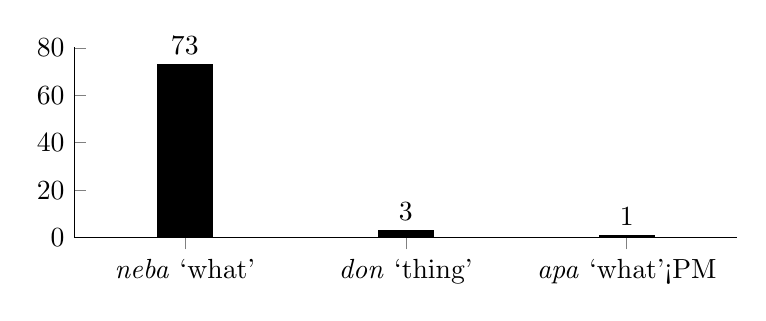
\begin{tikzpicture}
	\begin{axis}[ybar,
		axis lines*=left,
		nodes near coords,
		ymin=0,
		xtick={0,1,2},
		xticklabels={\textit{neba} `what',\textit{don} `thing',\textit{apa} `what'<PM},
		bar width=2em,
		enlarge x limits={0.25},
		height=4cm,
		width=10cm
		]
		\addplot [black, fill=black] coordinates {
			(0,73)
			(1,3)
			(2,1)
			};
	\end{axis}
  \end{tikzpicture}
  \caption{Frequency of placeholders.}\label{fig:ph}
% % % 	\includegraphics[width=\textwidth]{ph.png}
\end{figure}

\subsection{Frequency}
Figure~\ref{fig:phpers} shows that all six speakers that use placeholders use \textit{neba} `what'. The frequencies of the other placeholders are so low that one cannot meaningfully generalize.

\begin{figure}[ht]
% % % 	\includegraphics[width=\textwidth]{phpers.png}\\
	\begin{tikzpicture}
	\begin{axis}[ybar,
		axis lines*=left,
		nodes near coords,
		ymin=0,
		xtick={0,1,2},
		xticklabels={\textit{neba} `what',\textit{don} `thing',\textit{apa} `what'<PM},
		bar width=1em,
		enlarge x limits={0.25},
		height=4cm,
		width=\textwidth,
		cycle list name=langsci-RdYlBl-6,
		legend cell align=left,
		legend columns=3
		]
		\addplot+  coordinates {
			(0,11)
			(1,0)
			(2,0)
			};
		\addlegendentry{Fajara}
		\addplot+  coordinates {
			(0,15)
			(1,0)
			(2,1)
			};
		\addlegendentry{Hair}
		\addplot+  coordinates {
			(0,10)
			(1,0)
			(2,0)
			};
		\addlegendentry{Hawa}
		\addplot+  coordinates {
			(0,3)
			(1,1)
			(2,0)
			};
		\addlegendentry{Kamarudin}
		\addplot+  coordinates {
			(0,33)
			(1,0)
			(2,0)
			};
		\addlegendentry{Nurmia}
		\addplot+  coordinates {
			(0,1)
			(1,2)
			(2,0)
			};
		\addlegendentry{Sabtu}
	\end{axis}
  \end{tikzpicture}
	\caption{Usage of placeholders per speaker.}\label{fig:phpers}
\end{figure}

Placeholder \textit{neba} was previously reported to occur with a frequency of 6 per 1000 words in the full Kalamang corpus \citep[431]{visser2022}.\footnote{That means all narratives and conversations, including those prompted with some kind of stimulus material, but excluding elicitation sessions (which were not recorded at all). There are 104 texts of in total 69706 words, spoken by 25 speakers \citep[21, 28]{visser2022}. The list of texts can be found in Appendix C of \citet{visser2022}.} This frequency is higher in the current sample: $73/7416\times 1000 = 9.84$. If we also take into account the other placeholders, this ratio rises to 10.38 per 1000 words.

As for target retrieval, of the 73 instances of \textit{neba} `what', 25 times the target was retrieved (34.2\%) and 42 it was not (57.5\%). In the other 6 cases, it was unclear whether the target was retrieved or not. In the only example with \textit{apa} `what', the target was retrieved. In the three examples with \textit{don} `thing', no targets were retrieved. This is as expected, since \textit{don} is used to avoid expressing the target.

There are large inter-speaker differences in placeholder frequency, as presented in Table~\ref{tab:phspk}. While Hair uses more than 28 placeholders per 1000 words, Kamarudin does not even use four, and two speakers, Samsia and Bini, use no placeholders at all. See also \citet{chapters/ponsonnet} for differences between speakers, there described as differences in ``disfluency styles'', and \citet{chapters/pakendorf}, \citet{chapters/ventayol_boada} and \citet{chapters/mcdonnell_billings} for more obserservations on inter-speaker differences.

\begin{table}[ht]
	\caption{Placeholder ratio per 1000 words per speaker.}
	\label{tab:phspk}
		\begin{tabular}{lrrr}
			\lsptoprule
speaker& ratio  & words & placeholders \\
			\midrule
Hair &	28.42 &	563	& 16\\
Nurmia & 12.80 & 2579 & 33\\
Hawa&	10.74&	931	&10\\
Fajaria&	10.06	&1093&	11\\
Sabtu&	8.33&	360&	3\\
Kamarudin&	3.95&	1012&	4\\
Samsia&0&246&0\\
Bini&0&563&0\\\lspbottomrule
		\end{tabular}
\end{table}

\subsection{Discussion}
This study shows that \textit{neba} `what' is very much the preferred placeholder. This mirrors findings from e.g. English, where variants of one placeholder (\textit{thing(s)}, \textit{thingy} and \textit{thingie}) account for 75 to 87\% of all placeholder occurrences \citep{palacios2015} in four different corpora. The current study also reveals one instance of a borrowed placeholder: \textit{apa} `what' from Papuan Malay. This word is also used as a placeholder in Papuan Malay \citep[316]{kluge2017}. Like \textit{neba} `what', it has its origin in a question word, but it seems less morphosyntactically integrated in the Kalamang grammar than \textit{neba}, as in the one example it does not carry the inflection its target does (see \ref{exe:apaa} above).\footnote{In the entire Kalamang corpus, there are also a few instances of \textit{apa lagi}, which literally means `what else', but also `especially' in Indonesian and Papuan Malay. In the Kalamang corpus, it seems also to be used as a placeholder. There are no other clear examples of placeholder \textit{apa} in the entire Kalamang corpus.}

The adjusted frequency of placeholder \textit{neba} `what' from 6 in \citet{visser2022} to 9.84 here is likely due to two reasons: genre and more careful coding. In the current sample, only conversations were used. These are less planned in nature than narratives, which could possibly have an effect on placeholder use.\footnote{But see \citet{chapters/pakendorf} for an example of a supposedly excellent speaker who has a high frequency of fillers in fairy tales in Negidal. And in Mojeño Trinitario, traditional narratives show the highest rate of placeholders \citep{rosetalk}, often followed by a delayed constituent. %48 of presentation 
Because the content of traditional stories is known to the speaker and most of the addressees, the major challenge for the speaker is not their competence in remembering the content, but their performance in rendering the story, hence the many hesitations in looking for the best wording.} In earlier annotations, many uses of \textit{neba} as a placeholder were coded as instances of the question word. Taking into account also the three instances of \textit{don} `thing' and the instance of \textit{apa} `what', the placeholder ratio rises to 10.38. This is much higher than what was previously found in large well-studied languages. Russian has 5 per 1000 words in a corpus of informal elicited narratives (\citealt{podlesskaya2006} as cited in \citealt{podlesskaya2010}), and Mandarin has 6.68 per 1000 words in a corpus of telephone conversations \citep{zhao2005}. For English, frequencies are much lower still. \citet{palacios2015} find frequencies of 0.03 to 0.07 in four different conversational corpora. However, recent studies on lesser-known languages find higher ratios: the Evenki filler \textit{aŋi} has a frequency of 12.6 per 1000 words \citep{klyachko2022functions}, and \citet{chapters/pakendorf} finds 11.6 fillers (this includes both placeholders and hesitators) in Negidal. Combined with the Kalamang findings, this stresses the need for investigating placeholder frequencies in a wide range of languages.
 
\il{English}\il{Mandarin}\il{Russian}\il{Negidal}\il{Evenki}\il{Mojeño Trinitario}

Finally, we see large differences between speakers, which might boil down to differences in topic. Two of the eight speakers in the sample don't use placeholders at all. Note that these speakers' words form a small proportion of the total number of words (Samsia 3.3\%, Bini 7.6\%). Samsia has no other recordings in the entire Kalamang corpus, but there are five other recordings with Bini (both narratives and conversations). A quick search reveals that she uses \textit{neba} `what' as a placeholder five times in these recordings. A refined annotation might reveal more instances. On the other end of the scale is Hair, who has a ratio of 28.42, more than twice as high as number two, Nurmia. Like Samsia and Bini, in the sample he is represented with relatively few words, which all come from the same text. Hair is represented with other texts in the entire Kalamang corpus, but they are all narratives. In his longest narrative, which counts 1499 words, he does not use \textit{neba} `what' as a placeholder at all. An explanation for the high ratio in the present sample is that in the text (conv20), this speaker has great difficulties in retrieving the different herbal medicines that he knows, while the other speaker keeps urging him to do the talking. It was the researcher who requested the speakers to talk about herbal medicines. The topics of the other texts in the sample were determined by the speakers themselves. If we remove Hair from the sample, we are left with 61 placeholders and 6784 words, resulting in a ratio of 8.99 per 1000 words; still higher than what has been found in other languages.

\section{Hesitatives and other disfluencies}
\label{sec:hes}

\subsection{Overview of the forms}
Besides conventionalized \textit{nain} `like' (which is by far the most common with 37 instances): the sample also shows a high number of the less conventionalized \textit{a} `uh'\footnote{This spelling of the English hesitative \textit{uh}, \textit{er} or \textit{um} is used by for example Merriam-Webster (\url{https://www.merriam-webster.com/dictionary/uh)}.} (24 instances). Apart from these two hesitatives, there are three disfluency strategies for gaining time or marking problems with the planning and execution of speech: lengthening, mumbling and repetition. All hesitatives and other disfluencies are given with their frequencies in Figure~\ref{fig:hes}. There are 61 hesitatives and 34 other disfluencies in the corpus.

\begin{figure}[ht]
% % % 	\includegraphics[width=\textwidth]{hes.png}
  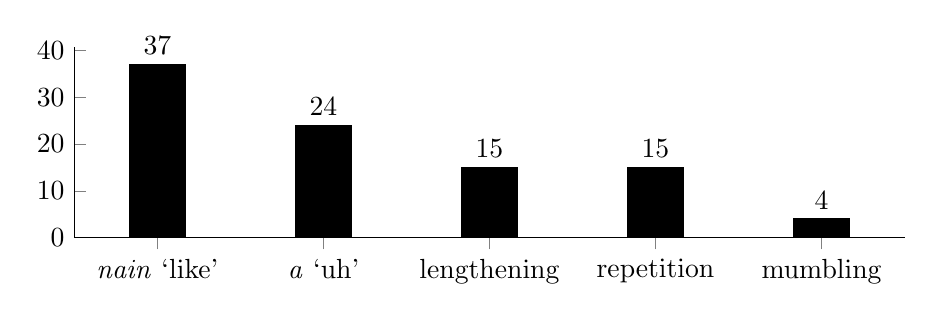
\begin{tikzpicture}
	\begin{axis}[ybar,
		axis lines*=left,
		nodes near coords,
		ymin=0,
		xtick={0,1,2,3,4},
		xticklabels={\textit{nain} `like',\textit{a} `uh',lengthening,repetition,mumbling},
		bar width=2em,
		enlarge x limits={0.125},
		height=4cm,
		width=\textwidth
		]
		\addplot [black, fill=black] coordinates {
			(0,37)
			(1,24)
			(2,15)
			(3,15)
			(4,4)
			};
	\end{axis}
  \end{tikzpicture}
	\caption{Frequency of hesitatives and other disfluencies.}\label{fig:hes}
\end{figure}

The sample shows that hesitatives with a more or less conventionalized form (\textit{nain} `like' and \textit{a} `uh') are much preferred to other strategies that mark disfluency.

\textit{Nain} `like' is the most frequent hesitative, and it is often used together with a placeholder. It is also not uncommon to have two instances of \textit{nain} in one utterance, like in (\ref{exe:munan}).

\ea \label{exe:munan}
\gll mu-nan \textbf{nain} opa \textbf{nain} neba-un me et kinkin=a saerak leng wa me\\
\textsc{3pl}-too like \textsc{ana} like what-\textsc{3poss} \textsc{top} canoe small=\textsc{foc} \textsc{neg.exist} village \textsc{prox} \textsc{top}\\
\glt `They too, like earlier, like whatsit, there are no small canoes in this village.'  \jambox*{\href{http://hdl.handle.net/10050/00-0000-0000-0004-1B93-C}{[conv14\_66]}}
\z

Then in the next utterance, the speaker possibly says what he really wanted to say:

\ea \label{exe:emumur}
\gll emumur et kinkinun me saerak\\
women canoe small \textsc{top} \textsc{neg.exist}\\
\glt `The women don't have small canoes.'  \jambox*{\href{http://hdl.handle.net/10050/00-0000-0000-0004-1B93-C}{[conv14\_67]}}
\z

Speakers can also start a turn with hesitative \textit{nain} `like', in the case of (\ref{exe:naina}) followed by hesitative \textit{a} `uh'. The pauses are indicated too, to show how much the speaker is struggling to formulate his thoughts.

\ea \label{exe:naina}
\gll \textbf{nain} \textbf{a} (0.6) opa (1.2) sontum (0.8) gier-un=at ning sontum mudamuda-ten gier-un=at tahan=et\\
like uh {} \textsc{ana} {} people {} tooth-\textsc{3poss=obj} ache people young-\textsc{at} tooth-\textsc{3poss=obj} last=\textsc{irr}\\
\glt `Like uh, before, people, whose teeth ache, young people who want to have lasting teeth...'  \jambox*{\href{http://hdl.handle.net/10050/00-0000-0000-0004-1BCA-4}{[conv20\_193--196]}}
\z 

(\ref{exe:tak}) illustrates \textit{a} `uh'. It is followed by a brief pause, after which the speaker continues with some production errors (\textit{se belum} `already not yet') before he lands on what he wants to say (\textit{pi tok muapnin} `we haven't eaten yet').

\ea 	\label{exe:tak}
\gll tak ramandalin-i jien terus \textbf{a} \textbf{(0.5)} me me se belum pi tok muap=nin\\
\textsc{clf\_leaf} seven-\textsc{objqnt} get then uh {} \textsc{dist} \textsc{top} {\glse} not\_yet \textsc{1pl.incl} still eat=\textsc{neg}\\
\glt 	`[You] get seven leaves, then, uh, that's when already, not yet, we haven't eaten yet.' \jambox*{\href{http://hdl.handle.net/10050/00-0000-0000-0004-1BCA-4}{[conv20\_166]}}
\z 

% (\ref{exe:len}) shows lengthening followed by a 2.2 second break before the speaker finishes his utterance.

% \ea 	\label{exe:len}
% \gll in war ba \textbf{piː} \textbf{(2.2)} et saerak=te\\
% \textsc{1pl.excl} fish but \textsc{1pl.incl} {} canoe \textsc{neg\_exist}=\glte\\
% \glt 	`We'd go fishing but we... there is no canoe.' \jambox*{\href{http://hdl.handle.net/10050/00-0000-0000-0004-1B93-C}{[conv14\_7:02]}}
% \z 

(\ref{exe:rep}) is an example of repetition, used in combination with the placeholder \textit{neba} `what'.

\ea 	\label{exe:rep}
\gll ge mena go \textbf{ma} \textbf{ma} \textbf{ma} neba\\
no otherwise condition \textsc{3sg} \textsc{3sg} \textsc{3sg} what\\
\glt 	`No otherwise it, it, it is whatsit?' \jambox*{\href{http://hdl.handle.net/10050/00-0000-0000-0004-1B9F-F}{[conv9\_298]}}
\z 

% Mumbling is rather infrequent and is only used by one speaker, exemplified in~(\ref{exe:mum}). The production difficulties are also visible from the fact that the speaker uses object-fronting, first with a full noun and then with a pronoun, and in both cases does not inflect the object with object marker \textit{=at}.

% \ea 	\label{exe:mum}
% \gll rorkiel \textbf{(mumbling)} ma pi jiet=et me\\
% root {} \textsc{3sg} \textsc{1pl.incl} get={\glet} {\glme}\\
% \glt 	`The root, it, we get...' \jambox*{\href{http://hdl.handle.net/10050/00-0000-0000-0004-1BCA-4}{[conv20\_2:08]}}
% \z 

The examples above show that hesitators and disfluencies may combine with pauses and other production difficulties, as well as placeholders (as in \ref{exe:munan} and \ref{exe:rep}). (\ref{exe:combi}) is a striking example that shows a combination of \textit{nain} `like', \textit{a} `uh' and \textit{neba} `what'.%\footnote{The word \textit{ah} is analysed as an `utterance divider' that indicates the speaker is moving on to the next step in the discourse, perhaps after having given some background information.}

\ea 	\label{exe:combi}
\gll terus \textbf{nain} \textbf{nain} sontum gier-un ning \textbf{a} gier-un ning \textbf{a} \textbf{neba} ah met me nain\\
then like like people tooth-\textsc{3poss} be\_sick uh tooth-\textsc{3poss} be\_sick uh what well \textsc{dist\_obj} {\glme} like\\
\glt 	`Then like, like, [when] people have a toothache, uh, a toothache, uh, whatsit, well that's like...' \jambox*{\href{http://hdl.handle.net/10050/00-0000-0000-0004-1BCA-4}{[conv20\_41]}}
\z 

\subsection{Frequency}
Figure~\ref{fig:hespers} shows that all types of disfluencies are used by all or most speakers that use them, except for mumbling, which is used by Hair only.

\begin{figure}
% % % 	\includegraphics[width=\textwidth]{hespers.png}\\
	\small
    \begin{tikzpicture}
	\begin{axis}[ybar stacked,
		axis lines*=left,
		nodes near coords,
		every node near coord/.append style={xshift=2em},
		ymin=0,
		xtick={0,1,2,3,4},
		xticklabels={\textit{nain} `like',\textit{a} `uh',lengthening,repetition,mumbling},
		bar width=3em,
		enlarge x limits={0.125},
		height=4cm,
		width=\textwidth,
		cycle list name=langsci-RdYlBl-6,
		legend cell align=left,
		legend columns=3
		]
		\addplot+ [every node near coord/.append style={anchor=base}] coordinates {
			(0,0)
			(1,1)
			(2,5)
			(3,2)
			(4,0)
			};
		\addlegendentry{Fajaria}
		\addplot+ [every node near coord/.append style={xshift=-4.2em}] coordinates {
			(0,27)
			(1,14)
			(2,5)
			(3,2)
			(4,4)
			};
		\addlegendentry{Hair}
		\addplot+ [nodes near coords={}] coordinates {
			(0,0)
			(1,0)
			(2,0)
			(3,1)
			(4,0)
			};
		\addlegendentry{Hawa}
		\addplot coordinates {
			(0,6)
			(1,3)
			(2,1)
			(3,5)
			(4,0)
			};
		\addlegendentry{Kamarudin}
		\addplot+ [every node near coord/.append style={xshift=-4.2em}] coordinates {
			(0,2)
			(1,5)
			(2,3)
			(3,4)
			(4,0)
			};
		\addlegendentry{Nurmia}
		\addplot coordinates {
			(0,2)
			(1,1)
			(2,1)
			(3,1)
			(4,0)
			};
		\addlegendentry{Sabtu}
	\end{axis}
  \end{tikzpicture}
	\caption{Usage of hesitatives and other disfluency strategies per speaker.}\label{fig:hespers}
\end{figure}

\begin{table}
	\caption{Hesitatives and other disfluencies ratio per 1000 words per speaker.}
	\label{tab:hesspk}
		\begin{tabular}{lrrr}
			\lsptoprule
			       &        &       & Hesitatives and\\
			Speaker& Ratio  & Words & other disfluencies\\
			\midrule
			Hair	    &92.36	&563	&52\\
			Kamarudin	&14.82&	1012	&15\\
			Sabtu	    &13.89	&360	&5\\
			Fajaria	    &7.32&	1093&	8\\
			Nurmia	    &5.43&2579&	14\\
			Hawa	    &1.07&	931&	1\\
			Samsia&0&246&0\\
			Bini&0&563&0\\\lspbottomrule
		\end{tabular}
\end{table}

\textit{Nain} `like' has a ratio of 4.99 per 1000 words, while \textit{a} `uh' has a ratio of 3.24 (compare with 4.01 for \textit{mm} and \textit{uh} in Mandarin; \citealt{zhao2005}).

There are large inter-speaker differences in the frequency of hesitative and other disfluency use, as presented in Table~\ref{tab:hesspk}. Hair uses more than 92 hesitatives per 1000 words, while the others score below 15. Two speakers, Samsia and Bini, use no hesitatives at all.

\subsection{Pronunciation}
There is quite some variation in the pronunciation of the hesitatives \textit{nain} and \textit{a}. Figure~\ref{fig:hesnainpron} shows the variation for \textit{nain} `like', showing that the majority of the utterances is [nɛin] followed by [nain]. It also shows that while [nɛin] (and a few other variants) are exclusively used by Hair, while (lengthened) [nain] is used by all four speakers who use this hesitative.

\begin{figure}[ht]
% % % 	\includegraphics[width=\textwidth]{hesnainpron.png}\\
	\small
\begin{tikzpicture}
	\begin{axis}[ybar stacked,
		axis lines*=left,
		cycle list name=langsci-RdYlBl-5,
		ymin=0,
		symbolic x coords={nɛin,nain,nainː,nin,ninː,nɛinː,nɛi,nː},
		xtick=data,
		ytick={0,2,...,18},
		height=6cm,
		width=\textwidth,
		legend cell align=left,
		legend columns=2,
		bar width=2em,
% % % 		nodes near coords, %% Alternative using grid
		every node near coord/.append style={xshift=1.6em},
		ymajorgrids=true
		]
		\pgfplotsset{cycle list shift=1} % Skip Fajara
		\addplot+ [every node near coord/.append style={yshift=2pt}] coordinates {
			(nɛin, 18)
			(nain, 1 )
			(nainː,0)
			(nin,  2 )
			(ninː, 2 )
			(nɛinː, 2)
			(nɛi, 1  )
			(nː, 1   )
			};
		\addlegendentry{Hair}
		\addplot+ coordinates {
			(nɛin, 0)
			(nain, 4)
			(nainː,2)
			(nin,  0 )
			(ninː, 0 )
			(nɛinː, 0)
			(nɛi, 0  )
			(nː, 0   )
		};
		\addlegendentry{Kamarudin}
		\addplot+ [every node near coord/.append style={xshift=-2.9em}] coordinates {
			(nɛin, 0)
			(nain, 1)
			(nainː, 1)
			(nin,  0 )
			(ninː, 0 )
			(nɛinː, 0)
			(nɛi, 0  )
			(nː, 0   )
		};
		\addlegendentry{Nurmia}
		\addplot+ coordinates {
			(nɛin, 0)
			(nain,1)
			(nainː,1)
			(nin,  0 )
			(ninː, 0 )
			(nɛinː, 0)
			(nɛi, 0  )
			(nː, 0   )
		};
		\addlegendentry{Sabtu}
	\end{axis}
\end{tikzpicture}
	\caption{Pronunciation variants of \textit{nain} `like'.}\label{fig:hesnainpron}
\end{figure}

Figure~\ref{fig:hesehpron} shows the pronunciations attested for \textit{a} `uh'. By far the most common pronunciation is [aː], and it is used by four of the five speakers who use this hesitative.\footnote{Kalamang also has an utterance divider \textit{ah}. Its function seems to have something to do with structuring the discourse, akin to English conjunctions like `and then' or `so'. The utterance divider is always pronounced as [a] (not lengthened), followed by a brief pause. It always occurs utterance-initially. An example can be found in the last part of \REF{exe:combi}.}

\begin{figure}[ht]
% % % 	\includegraphics[width=\textwidth]{hesehpron.png}\\
	\small
	\begin{tikzpicture}
	\begin{axis}[ybar stacked,
		axis lines*=left,
		cycle list name=langsci-RdYlBl-5,
		ymin=0,
		symbolic x coords={aː,əː,aːh,e,eː,məː,mː,oəː,əːhm},
		xtick=data,
		ytick={0,2,4,...,12},
		height=5cm,
		width=\textwidth,
		legend cell align=left,
		legend columns=2,
		bar width=2em,
		nodes near coords,
		yminorgrids=true,
		ymajorgrids=true
	]
		\addplot coordinates {
			(aː, 1)
			(əː, 0)
			(aːh,0)
			(e,0)
			(eː,0)
			(məː,0)
			(mː,0)
			(oəː,0)
			(əːhm, 0)
			};
		\addlegendentry{Fajaria}
		\addplot coordinates {
			(aː, 8)
			(əː, 4)
			(aːh,1)
			(e,0)
			(eː,0)
			(məː,0)
			(mː,0)
			(oəː,0)
			(əːhm, 1)
			};
		\addlegendentry{Hair}
		\addplot+ coordinates {
			(aː, 1)
			(əː, 1)
			(aːh,1)
			(e,0)
			(eː,0)
			(məː,0)
			(mː,0)
			(oəː,0)
			(əːhm, 0)
		};
		\addlegendentry{Kamarudin}
		\addplot coordinates {
			(aː, 0)
			(əː, 0)
			(aːh,0)
			(e,1)
			(eː,1)
			(məː,1)
			(mː,1)
			(oəː,1)
			(əːhm, 0)
		};
		\addlegendentry{Nurmia}
		\addplot coordinates {
			(aː, 1)
			(əː, 0)
			(aːh,0)
			(e,0)
			(eː,0)
			(məː,0)
			(mː,0)
			(oəː,0)
			(əːhm, 0)
		};
		\addlegendentry{Sabtu}
	\end{axis}
\end{tikzpicture}
	\caption{Pronunciation variants of \textit{a} `uh'.}\label{fig:hesehpron}
\end{figure}

\subsection{Discussion}
This study has confirmed \textit{nain} `like' as the main hesitative. This word originally denotes similarity or attribution to a class, just like the hesitative \textit{like} in English \citep{laserna2014like} or \textit{tipa} in Russian \citep{egorova2018}. The grammaticalization path from simile to quotative is well-attested across the world's languages \citep[274]{heinekuteva2002}. From there, it is a small step into being pragmaticized into a word search marker or a hesitative  (Vera Podlesskaya, p.c.). Note that Kalamang \textit{nain} `like' is not attested as a quotative, though, so perhaps we should propose a direct path from simile to hesitative. The opposite development is attested in Udi and Agul \citep[111]{ganenkovetal2010}. 

The frequency count has established \textit{a} `uh' as another important hesitative. Previously, it was transcribed only sporadically in the Kalamang corpus due to a lack of awareness. Like \textit{huh?}, a questioning interjection for other-initiation of repair, \textit{a} `uh' might be a universal hesitative with cross-linguistically very similar pronunciation, namely with the articulators in near-neutral position \citep{dingemanse2013}. Similar forms have been discussed for English, Dutch and German \citep{clark2002using, leeuw2007hesitation}. If \textit{uh} is truly universal, then this form, like \textit{huh?}, might be the result of convergent cultural evolution, reflecting ``selective pressure towards the evolution of common optimised forms'' \citep[e78273]{dingemanse2013}.\il{English}\il{Dutch}\il{German}

The differences between speakers in frequency of hesitative use can likely again be explained by the topic of conversation. Like for the placeholders, Hair has a very high frequency, likely again due to the fact that he is constantly scraping his memory for medicines to discuss.

The breakdown of the two hesitatives into pronunciation variants and by speaker can inform choices in the development of a standardised spelling by choosing the spelling that is closest to the most common pronunciation. While [nɛin] is the most common pronunciation for \textit{nain} `like', it is only used by one speaker in the subset of the corpus. If we collapse lengthened and non-lengthened pronunciations, there are 19 instances of [nɛin], all by the same speaker, while there are 11 instances of [nain] by all four speakers that use this hesitative. It seems therefore best to spell this hesitative as \textit{nain}. \textit{A} `uh' mainly has the pronunciation variants [a], [e] and [ə] and the consonants [m] and [h]. The latter only occurs in interjections in Kalamang, not in other word classes. The pronunciation [a] is used by four of the five speakers that use this hesitative, so \textit{a} seems to be the best spelling for `uh' based on this sample. While native speakers might not be interested in the spelling of a hesitative like \textit{a} `uh', since they would not write it anyway, they certainly write the conventionalized form \textit{nain} `like'. In addition, this kind of analysis helps choosing the best spelling when transcribing recordings for linguistic use, a task for which it is common to train native speakers \citep[62]{chelliah2013fieldwork}. However, to make a final decision about the spelling of these items, one would need to look at more data first, as this analysis is based on very few items and four or five speakers.


\section{Conclusion}
\label{sec:concl}
Despite the small sample of the Kalamang corpus used for this study, it has contributed to further understanding of Kalamang fillers. We have seen that the ratio of placeholders is higher in this sample than in the entire Kalamang corpus, which is partly due to better transcription and glossing, but may also have been affected by the choice of genre (conversations, excluding narratives) and by individual speakers. This stresses the need for (language documentation) corpora that contain many genres and speakers \citep[46--47]{woodbury2003}, and for being explicit about these parameters in studies that use (parts of) these corpora. 

The higher ratio of placeholders in the current sample may also have been affected by the topics represented. The text with most hesitatives and placeholders is about a topic that one of the speakers did not find so easy to talk about, namely medicines made from plant roots (conv20). Since this was also one of the longer texts, this might have affected the ratio of fillers, but note that the ratio of placeholders in the sample is still higher than what has been found in other languages when removing this one speaker, namely 8.99 per 1000 words. It can be hypothesized that talking about less familiar topics, or a topic one is not well-prepared for (in the case of the root medicine conversation) triggers the use of more fillers. This could be further investigated experimentally, for example with a picture matching task with pictures of familiar and unfamiliar objects. Earlier research \citep{rosetalk} found no use of placeholders at all in rehearsed genres and very few placeholders in stimulus-based fiction, also indicating that familiarity with the topic or planning plays a role.

The refined coding of hesitatives in the current sample has revealed that \textit{a} `uh', analysed before as a ``filler interjection" \citep[148]{visser2022}, is a quite common hesitative. This is not surprising, as such a hesitative may be a universal feature of languages \citep{dingemanse2013}. 

Another finding is that some speakers seem to use placeholders more often than hesitatives. Nurmia, Hawa and Fajaria all use more placeholders than hesitatives, while it is the other way around for Hair, Sabtu and Kamarudin (see Table~\ref{tab:ph+hesspk}). At least for Russian, there is data suggesting that hesitatives, especially non-lexical ones, are much more frequent than placeholders \citep{kibrik2009}.\footnote{\citet{chapters/pakendorf} also finds inter-speaker variation in the frequency of placeholders versus hesitatives in her Negidal corpus, but all speakers use placeholders more frequently than hesitatives. Note, however, that these results are not entirely comparable to the Kalamang data because she only regards the placeholder versus hesitative uses of a single filler, and disregards the `uh' hesitative.} There is no good explanation for this difference at the moment, but note that all women use more placeholders, while all men use more hesitatives. So for now, we can only hypothesise that there is a gender difference in the relative frequency of placeholders and hesitatives.

\begin{table}[h!]
	\caption{Placeholder and hesitative ratio per 1000 words per speaker.}
	\label{tab:ph+hesspk}
		\begin{tabular}{lrrr}
			\lsptoprule
            Speaker& Placeholder ratio & Hesitative ratio  & Words \\
			\midrule
            Hair &	28.42 &	92.36 & 563\\
            Nurmia & 12.80 & 5.43 & 2579\\
            Hawa & 10.74& 1.07 & 931\\
            Fajaria & 10.06 & 7.32 & 1093\\
            Sabtu &	8.33 &	13.89 & 360\\
            Kamarudin &	3.95 & 14.82 & 1012\\
            Samsia&0&0 & 246\\
            Bini&0&0 & 563\\\lspbottomrule
		\end{tabular}
\end{table}


Finally, analysing the pronunciation of hesitatives and other ``peripheral'' words like interjections, which often show more variation in pronunciation than other words, can inform the development of a standardised spelling in language documentation projects.

\section*{Acknowledgments}
I would like to thank the editors of this volume for several rounds of very careful reviewing, which greatly improved the quality of this chapter.

\section*{Abbreviations}
\begin{tabularx}{.5\textwidth}[t]{@{}lQ@{}}
\textsc{ana} & anaphoric demonstrative \\
\textsc{at} & attributive \\
\textsc{atten} & attenuative \\
\textsc{clf\_leaf} & classifier for thin flat entities\\
\textsc{com} & comitative\\
\textsc{dist} & distal\\
\textsc{emph} & emphasis \\
\textsc{excl} & exclusive\\
\textsc{exist} & existential \\
\textsc{foc} & focus\\
\textsc{iam} & iamitive\\
\textsc{incl} & inclusive\\
\textsc{int} & interjection\\
\textsc{irr} & irrealis\\
\end{tabularx}%
\begin{tabularx}{.5\textwidth}[t]{@{}lQ@{}}
\textit{lat} & ablative/allative\\
\textsc{loc} & locative\\
\textsc{neg} & negator \\
\textsc{nfin} & nonfinal \\
\textsc{obj} & object \\
\textsc{objqnt} & object quantifier \\
\textsc{pl} & plural\\
\textsc{plnk} & predicate linker \\
\textsc{poss} & possessive\\
\textsc{prox} & proximal\\
\textsc{sg} & singular\\
\textsc{sim} & similative\\
\textsc{tag} & tag \\
\textsc{top} & topic\\
\end{tabularx}

%\section*{Acknowledgements}

%\section*{Contributions}
%John Doe contributed to conceptualization, methodology, and validation. 
%Jane Doe contributed to writing of the original draft, review, and editing.

\sloppy
\printbibliography[heading=subbibliography,notkeyword=this]
\end{document}
